% SPDX-FileCopyrightText: 2023 SAP SE
%
% SPDX-License-Identifier: Apache-2.0
%
% This file is part of FEDEM - https://openfedem.org

%%%%%%%%%%%%%%%%%%%%%%%%%%%%%%%%%%%%%%%%%%%%%%%%%%%%%%%%%%%%%%%%%%%%%%%%%%%%%%%%
%
% FEDEM User Guide.
%
%%%%%%%%%%%%%%%%%%%%%%%%%%%%%%%%%%%%%%%%%%%%%%%%%%%%%%%%%%%%%%%%%%%%%%%%%%%%%%%%

\Section{Joints}{joints}

As with real mechanisms, you may connect one part or beam to another using
{\sl joints}. A joint introduces motion and/or spring constraints between the
two parts it is acting between. These constraints are applied on the
{\sl joint DOFs}, also called {\sl Joint Variables}.
Each Fedem joint uses at least two triads to connect the joint to parts.
One or more of the joint's triads are labeled {\sl master} while one triad
is labeled {\sl slave}, with the constrained DOFs of the slave triad following
the movement of the master(s).
(See the \FedemTGuide{Chapter 6, "Modeling of Joints"}.)

To attach a joint to parts, the joint's master triad is attached
to an FE node on one part and the slave triad to an FE node on another part.
This means that when the mechanism moves, the FE node (and part) on the slave
side of the joint follows the motion of those on the master side.
FE nodes and parts can, therefore, also be referred to as masters and slaves.
See \refSection{attaching-and-detaching-elements}
{Attaching and detaching elements} and
\refSection{using-the-attach-command}{Using the Attach command}
about how to attach joints.

\Tip{To determine which triad is the master and which is the slave,
  select one of the parts or the joint to examine the {\sl Topology} view
  of master and slave triads connected to the part/joint.
  You can then select (click and hold down the mouse button) the master/slave
  triad to highlight it in the Modeler view.}


%%%%%%%%%%%%%%%%%%%%%%%%%%%%%%%%%%%%%%%%%%%%%%%%%%%%%%%%%%%%%%%%%%%%%%%%%%%%%%%%
\SubSection{Joint variables}{joint-variables}

The joint variables are the accessible or controllable DOFs for each joint.
As an example, the Revolute Joint normally has one accessible DOF,
namely the rotation about one axis. The other DOFs are fixed.
For most joints the DOFs that are not accessible are fixed,
but for Prismatic and Cylindrical joints that is not the case.
Refer to \protect\hyperlink{prismatic-joint}{\sl"Prismatic joint"} and
\protect\hyperlink{cylindric-joint}{\sl"Cylindric joint"} for further details.

The behavior of the joint variable can be controlled or customized in
several ways. There are four main options.

\begin{itemize}
\item{\sl Fixed} --
  This DOF is fixed, and can not be moved.
  It is removed from the system of equations (condensed out).
\item{\sl Free} --
  This DOF is free to move. No constraints are applied.
\item{\sl Prescribed} --
  This DOF can be assigned a prescribed motion,
  and is thus condensed out from the system of equations.
\item{\sl Spring-Damper} --
  This DOF is free to move, but a spring and a damper may be applied
  to assign stiffness and/or damping properties to it.
\end{itemize}


\subsubsection{Integrated springs and dampers}

When setting a joint variable to be spring and damper controlled,
the joint springs and joint dampers are initially inactive (their properties---
including spring stiffness and damper coefficient---are initially set to zero).
You can then assign values to the joint's spring and damper properties in the
Property Editor panel (see
\refSection{springs-and-dampers}{Springs and Dampers}
for more information about the spring and damper behavior.)

The integrated springs and dampers are listed in the {\sl Topology} view of the
joint as separate items; they are however not listed in the {\sl Objects} list
of the Model Manager. You can access the full Property Editor panel for the
joint springs and dampers by double-clicking on the entry in the {\sl Topology}
view, but the normal way of editing their properties is through the DOF tabs
in the Joint Property Editor panel (see
\protect\hyperlink{joint-variable-properties}{\sl"Joint variable properties"}
below).


%%%%%%%%%%%%%%%%%%%%%%%%%%%%%%%%%%%%%%%%%%%%%%%%%%%%%%%%%%%%%%%%%%%%%%%%%%%%%%%%
\SubSection{Joint properties}{joint-properties}

You can select a joint to display its properties in the {\sl Property Editor}
panel (shown below for a Free joint). For all joint types, the panel consists of
one tab with a summary table of the major joint properties, and additional tabs
for each of the {\sl joint variables} where their properties are displayed in
detail. The summary table shows a non-editable summary of all joint variables
along with other editable joint properties.
There is an {\sl Origin} tab for the point-to-point joint types
(Rigid, Revolute, Ball and Free joints) and an {\sl Advanced} tab with further
properties for Ball and Free joints.
Finally, all joint types (except for Rigid joints) have a {\sl Results} tab
for output specification.

Since the number of joint variables depends on the joint type, you may see from
zero (Rigid joint) to six (Free joint) sets of joint variables listed in the
summary table and a similar number of joint variable tabs.

\begin{figure}[H]
  \begin{picture}(343,104)
    \put(0,-7){\includegraphics[width=\textwidth]{\ReferenceImg/prp/free-joint-1}}
    \put(15,103){\Bullet{1}}
    \put(43,103){\Bullet{2}}
    \put(105,103){\Bullet{3}}
    \put(178,103){\Bullet{4}}
    \put(207,103){\Bullet{5}}
    \put(30,5){\Bullet{6}}
    \put(250,15){\Bullet{7}}
  \end{picture}
\end{figure}

\begin{bulletlist}
\item{\sl Summary tab} --
  This tab displays a \protect\hyperlink{summary-table}{\sl Summary table}
  over all properties of the selected joint.

\item{\sl Origin tab} --
  This tab contains the definition of the joint coordinate system, i.e.,
  the position and orientation of its origin
  (see \refSection{origin-property}{Origin property}).
  The joint variables are defined in this coordinate system. See also
  \refSubSection{moving-point-to-point-joints}
                {Moving point-to-point joints}
                {point-to-point-joints}.

\item{\sl Joint variable tabs} --
  These tabs display the propertie related to the joint variable in question
  (see \protect\hyperlink{joint-variable-properties}
  {\sl"Joint variable properties"} below).

\item
  {\sl Advanced tab} --
  This tab displays properties related to rotation formulation and spring
  inter-connectivity of the joint (see
  \protect\hyperlink{advanced-joint-properties}{\sl"Advanced joint properties"}
  below).

\item{\sl Results tab} --
  This tab contains toggles for activating output of certain solution variables
  related to the joint,
  see \protect\hyperlink{joint-results-tab}{\sl"Results tab"} below.

\item{\sl Friction} --
  Some joint types allow you to add friction properties to the joint
  by selecting from the list of frictions in your model (see
  \refSection{frictions}{Frictions}).

\item
  {\sl Set All Free/Fixed} --
  These two buttons enables you to quickly set the Constraint type of all the
  joint DOFs to either {\sl Free} or {\sl Fixed},
  without the need to go into each of the joint DOF tabs.
\end{bulletlist}


\SubSubSection{Joint variable properties}{joint-variable-properties}

The joint variable tabs display the different options and settings for each
joint variable. The displayed options depend on the {\sl Constraint Type}.

\SubSubSection{\sl\textbf{Free}}{free-joint-var}

\begin{figure}[H]
  \begin{picture}(343,80)
    \put(0,0){\includegraphics[width=\textwidth]{\ReferenceImg/prp/joint-2}}
    \put(46,53){\Bullet{1}}
    \put(40,16){\Bullet{2}}
    \put(60,2){\Bullet{3}}
    \put(190,58){\Bullet{4}}
    \put(200,22){\Bullet{5}}
  \end{picture}
\end{figure}

\begin{bulletlist}
\item{\sl Additional BC} --
  When this toggle is enabled, the movement in this joint variable is fixed
  during the initial equilibrium analysis and optionally also in the eigenmode
  analysis. (See also
  \refSubSection{eigenmode-tab}{Eigenmode tab}{dynamics-solver-advanced-mode}
  and the \FedemTGuide{Section 7.8, "Quasistatic equilibrium"}
  and {\sl Section 9.6, "Eigenvalue results"}.)

\item{\sl Load magnitude} --
  You can apply a {\sl Load} on the joint variable.
  This will be a torque or a force depending on whether the joint variable
  is a translational or a rotational DOF. The actual force value will be saved
  as a results quantity and thus available for plotting in a graph.

\item
  {\sl Initial velocity} - You may specify a velocity that should be
  applied as initial condition in this joint variable, i.e., the actual
  velocity at the start time of the dynamics simulation.

  \Note{The initial velocities of the slave triad in a joint are derived
    automatically in Fedem from the initial velocities of the joint DOFs and
    the master triad(s), based on the constraint equations representing the
    joint. However, it is also possible to specify the slave triad
    velocities explicitly and leave the joint DOF velocities zero.
    Fedem will then derived the initial joint DOF velocities by inverting the
    constraint equations of the joint. If non-zero initial velocities are
    specified in both the joint DOFs and slave triad DOFs, only the joint
    DOF values are used.}
\item
  {\sl Length/Angle in model} - This field shows the initial value of
  this joint variable as modeled. The value defines the initial
  configuration of this joint variable in the dynamics simulation. For
  rotational DOFs the value can be edited to set a different initial rotation.
  The 3D view will then update instantly, showing the new rotation in the joint
  symbol.
\item
  {\sl Apply in frequency domain} -- If a {\sl Function} is specified
  in the {\sl Load magnitude} field, this toggle will enable the load
  to be applied in the frequency domain instead of the time domain,
  if the {\sl Frequency response analysis} toggle is enabled in the
  Dynamics Solver Setup dialog box,
  see \refSection{dynamics-solver-basic-mode}{Dynamics Solver (Basic Mode)}.
\end{bulletlist}

\subsubsection{\sl\textbf{Fixed}}

\begin{figure}[H]
  \begin{picture}(343,75)
    \put(0,0){\includegraphics[width=\textwidth]{\ReferenceImg/prp/joint-3}}
    \put(190,55){\Bullet{1}}
  \end{picture}
\end{figure}

\begin{bulletlist}
\item{\sl Length/Angle in model} --
  This field shows the fixed value of this joint variable as modeled.
  For rotational DOFs the value can be edited to set a different fixed rotation
  state. The 3D view will then update instantly,
  showing the new rotation in the joint symbol.
\end{bulletlist}

\Tip{You may plot the reaction force associated with a fixed joint DOF by
  selecting the {\rm Force/Moment value} item under the joint variable node
  in question from the RDB selector (see
  \refSubSection{selecting-rdb-results}{Selecting RDB results}
                {curve-properties}).}

\subsubsection{\sl\textbf{Prescribed}}

\begin{figure}[H]
  \begin{picture}(343,80)
    \put(0,0){\includegraphics[width=\textwidth]{\ReferenceImg/prp/joint-4}}
    \put(40,15){\Bullet{1}}
    \put(60,3){\Bullet{2}}
    \put(170,59){\Bullet{3}}
    \put(170,40){\Bullet{4}}
    \put(125,10){\Bullet{5}}
    \put(220,13){\Bullet{6}}
  \end{picture}
\end{figure}

\begin{bulletlist}
\item{\sl Prescribed quantity} --
  You may choose whether you want to prescribe the {\sl Deflection},
  the {\sl Velocity} or the {\sl Acceleration} for the joint DOF.

\item{\sl Initial velocity} --
  You may specify a velocity that should be applied as initial condition in this
  joint variable, i.e., the velocity at the start time of
  the dynamics simulation.

\item{\sl Length/Angle in model} --
  This field shows the initial value of this joint variable as modeled,
  and has the same interpretation as when the joint variable is
  \protect\hyperlink{free-joint-var}{\sl Free} (see above).

\item{\sl Constant length/angle, Constant displacement/rotation} --
  These radio buttons and fields work together to allow you to set a constant
  prescribed value of the joint variable during the dynamics simulation.
  You can choose to enter the constant length/angle either as an absolute value,
  or relative to the {\sl Length/angle in model},
  if the {\sl Prescribed quantity} is set to {\sl Deflection}.
  For prescribed {\sl Velocity} or {\sl Acceleration}, you enter the constant
  velocity/acceleration that should be applied in the first of these two fields
  (the other field is inactive).

\EnumCaution{If you prescribe a {\rm length/angle} that differs from the
  {\rm Length/Angle in model}, this difference will be accounted for in the very
  first iteration of the dynamics simulation and thus lead to a dynamic shock
  effect. However, when the initial
  \protect\hyperlink{static-equilibrium-analysis}
                    {\sl Static equilibrium analysis}
  is switched on, the force due to this difference is taken as a pure static
  load and the transient shock should be avoided.}

\item{\sl Length/Angle change} --
  You can prescribe the evolution of the motion during the simulation through
  a function. The function controls the {\sl change} of the variable relative to
  the {\sl Constant length/angle}, or the change of the velocity/acceleration
  relative to the {\sl Constant velocity/acceleration},
  in case {\sl Velocity} or {\sl Acceleration} is prescribed.

\item{\sl Apply in frequency domain} --
  If a {\sl Function} is specified in the {\sl Length/Angle change} field,
  this toggle will enable the prescribed motion to be applied in the frequency
  domain instead of the time domain, if the {\sl Frequency response analysis}
  toggle is enabled in the Dynamics Solver Setup dialog box, see
  \refSection{dynamics-solver-basic-mode}{Dynamics Solver Basic Mode}
\end{bulletlist}

\Tip{You may plot the reaction force associated with a fixed joint DOF by
  selecting the {\rm Force/Moment value} item under the joint variable node in
  question from the RDB selector (see
  \refSubSection{selecting-rdb-results}{Selecting RDB results}
                {curve-properties}).}

\subsubsection{\sl\textbf{Spring-Damper}}

\begin{figure}[H]
  \begin{picture}(343,80)
    \put(0,0){\includegraphics[width=\textwidth]{\ReferenceImg/prp/joint-5}}
    \put(50,52){\Bullet{1}}
    \put(43,17){\Bullet{2}}
    \put(60,3){\Bullet{3}}
    \put(160,70){\Bullet{4}}
    \put(270,70){\Bullet{5}}
    \put(270,38){\Bullet{6}}
  \end{picture}
\end{figure}

These options enable you to add elastic and damping
behavior to the joint variable by entering values for the spring
and damper properties.

\begin{bulletlist}
\item{\sl Additional BC} --
  When this toggle is enabled, the movement in this joint variable is fixed
  during the initial equilibrium analysis and optionally also in the eigenmode
  analysis. It has the same interpretation as when the joint variable is
  \protect\hyperlink{free-joint-var}{\sl Free} (see above).

\item{\sl Load magnitude } --
  You can apply a Load in the joint variable, similarly as when the joint
  variable is \protect\hyperlink{free-joint-var}{\sl Free} (see above).

\item{\sl Initial velocity} --
  You may specify a velocity that should be applied as initial condition
  in this joint variable, similarly as when the joint variable is
  \protect\hyperlink{free-joint-var}{\sl Free} (see above).

\item{\sl Stress free length/angle control} --
  This group of options concerns spring deflection calculation similar to the
  {\sl Length/Angle control} of a {\sl Prescribed} joint variable.
  See also \refSection{spring-properties}{Spring properties}.

\item{\sl Spring properties} --
  This group of options concerns the spring characteristics,
  namely the relation between deflection and force.
  See \refSection{spring-properties}{Spring properties} for details.

\item{\sl Damper force/coefficient} --
  This group of options concerns the damper characteristics,
  namely the relation between velocity and force.
  See \refSection{damper-properties}{Damper properties} for details.
\end{bulletlist}


\SubSubSection{Summary table}{summary-table}

The summary table displays an overview of the settings for each joint variable.
The columns relate to the fields in the
\protect\hyperlink{joint-variable-properties}{\sl Joint variable properties}
described above.

\begin{figure}[H]
  \includegraphics[trim=0 15.2 0 0,clip,width=\textwidth]{\ReferenceImg/prp/free-joint-1}
\end{figure}

\begin{itemize}
\item{\sl Constraint} --
  Shows the {\sl Constraint type} selected for the joint variable.
\item{\sl Load} --
  Shows the load applied to the joint variable.
\item{\sl Model length} --
  Shows the modeled length/angle of the joint variable.
\item{\sl Init disp.} --
  Shows the initial deflection set up for the joint variable.
\item {\sl Length change} --
  Displays the function, if any, that controls the change of length/angle
  of the joint variable. If the constraint type is set to {\sl Prescribed} this
  change is directly applied to the joint DOF. If the Constraint type is set to
  {\sl Spring-Damper}, however, this function controls the
  {\sl Stress free length/angle change} of the spring.
\item{\sl Init vel.} --
  Shows the initial velocity applied to the joint variable.
\item{\sl Spring} --
  Displays the spring characteristics of the joint variable.
  Either a number describing a constant stiffness of the spring,
  or a description of the spring characteristics used as a non-linear
  stiffness- or force-deflection relationship.
\item{\sl Spr. scale} --
  Displays the function that is used to scale the force developed in the spring.
  Empty if no scaling is specified.
\item{\sl Damper} --
  Displays the damping characteristics of the joint variable.
  Either a number describing a constant damping coefficient, or a description of
  a function used as a non-linear coefficient- or force-velocity relationship.
\item{\sl Dmp. scale} --
  Displays the function that is used to scale the force developed in the damper.
  Empty if no scaling is specified.
\end{itemize}


\SubSubSection{Advanced joint properties}{advanced-joint-properties}

For the Ball joint and Free joint, you have possibility to alter the
numerical formulation of how the
rotational DOFs are represented internally. You can also control the
{\sl spring inter-connectivity}, a feature that can be used to describe
the circular or cylindrical stiffness behavior of rubber bushings, etc.
This is done through the {\sl Advanced} tab shown below.

\begin{figure}[H]
  \begin{picture}(343,83)
    \put(0,0){\includegraphics[width=\textwidth]{\ReferenceImg/prp/joint-6}}
    \put(-10,49){\Bullet{1}}
    \put(-10,36){\Bullet{2}}
    \put(290,55){\Bullet{3}}
  \end{picture}
\end{figure}

\begin{bulletlist}
\item You may change the rotational formulation of the joint.
  The following choices are available:
  \begin{itemize}
  \subitem{\sl Sequential rotation, Follower axis} :
    Euler angle parametrization.
  \subitem{\sl Sequential rotation, Orthogonal axis} :
    Euler angle parametrization.
  \subitem{\sl Rotational vector} :
    Singularity free Rodriguez parametrization.
  \end{itemize}
  See the \FedemTGuide{Section 2.3, "Finite rotations"}
  for further details on these choices.

\item You may alter the update sequence of the Euler angle parameters.
  The default sequence is Z-Y-X.

\EnumCaution{The Sequential rotation
    formulation may lead to singularities in the rotation update
    computations if the joint undergoes a 90 degrees
    rotation about the local $Y$-axis. If you have such behavior in the joint,
    you must use the Rotational vector formulation to achieve proper
    results.}

\item You may specify how the translational- and rotational joint springs
  should be inter-connected (Cylindrical or Spherical coordinates).
  This can be used to describe the cylindrical or spherical behavior of rubber
  bushings, or pin joints with clearances. If you want the spring
  characteristics in the joint variables to be interpolated resulting
  in a cylindrical/spherical behavior, select the proper setting from the
  drop-down menu. Please refer to the
  \FedemTGuide{Section 5.1.1, "Interconnected Spring Elements"}
  for details on how this affects the stiffness matrix.
\end{bulletlist}


\SubSubSection{Results tab}{joint-results-tab}

\begin{figure}[H]
  \begin{picture}(343,83)
    \put(0,0){\includegraphics[width=\textwidth]{\ReferenceImg/prp/joint-7}}
    \put(65,70){\Bullet{1}}
    \put(210,70){\Bullet{2}}
    \put(300,70){\Bullet{3}}
  \end{picture}
\end{figure}

The {\sl Results} tab (shown above) contains toggles for activating
output of secondary solution variables to the results database for the
selected joint, such that they are available for curve plotting, etc.

\begin{bulletlist}
\item{\sl Joint variables} --
  Activates output of the respective solution variables associated with
  each DOF in the joint.
\item{\sl Spring variables} --
  Activates output of the respective spring quantities in each
  spring/damper-constrained DOF in the joint. These toggles are not present
  if none of the joint DOFs are spring/damper-constrained.
\item{\sl Damper variables} --
  Activates output of the respective damper quantities in each
  spring/damper-constrained DOF in the joint. These toggles are not present
  if none of the joint DOFs are spring/damper-constrained.
\end{bulletlist}

\Tip{You don't need to enable these toggles if the solver option
  {\tt-allSecondaryVars} or {\tt-allJointVars} is used.
  Then these quantities will be stored for all joints in the model.}


%%%%%%%%%%%%%%%%%%%%%%%%%%%%%%%%%%%%%%%%%%%%%%%%%%%%%%%%%%%%%%%%%%%%%%%%%%%%%%%%
\SubSection{Point-to-point joints}{point-to-point-joints}

\begin{minipage}{0.75\textwidth}
  \raggedright
  With point-to-point joints, the motion constraints of the joint are applied
  between two points represented by the slave and the master triad with
  their corresponding FE nodes. Point-to-point joints are found on the
  \textbf{Mechanism Creation} tool bar (shown at right).
\end{minipage}% <--- the % is needed here to kill off spurious spacing
\hfill\begin{minipage}{0.2\textwidth}
\includegraphics[width=\textwidth]{Figures/1st_Joint_Pulldown}
\end{minipage}

Each of the point-to-point joint types are described in the following.


\subsubsection{Revolute joint}

\IconTextFirst{revoluteJoint}{
  The revolute joint has a single DOF that allows rotation of one part with
  respect to another about a common axis. Its joint variable is the angle
  from the master triad to the slave triad about the common $Z$-axis
  (defined by the right-hand rule).}

\begin{wrapfigure}[3]{r}{0.25\textwidth}
  \includegraphics[width=0.25\textwidth]{Figures/4-ZtranslationDOF}
\end{wrapfigure}

The Revolute joint has an optional Joint variable too; namely the translation
along the common $Z$-axis. This Joint variable can be toggled on or off on the
{\sl Summary} tab of the Revolute joint Property Editor panel.

\begin{wrapfigure}[10]{r}{0.33\textwidth}
  \begin{picture}(112,120)
    \put(-5,0){\includegraphics[width=0.35\textwidth]{Figures/revoluteJoint}}
    \put(65,48){\Bullet{1}}
    \put(101,63){\Bullet{2}}
    \put(18,105){\Bullet{3}}
  \end{picture}
\end{wrapfigure}

The symbol for a revolute joint is displayed in the {\sl Modeler} view
as shown to the right.

\begin{bulletlist}
\item The arrow represents the slave triad and indicates the positive direction
  for the joint angle.
\item The straight line (labeled $X$) represents the master triad.
\item The revolute axis is the common $Z$-axis of the master and slave triads.
  Together with the circle it represents the joint itself.
\end{bulletlist}

You can add friction to a revolute joint by selecting one from the list
of frictions in your model in the {\sl Friction} pull-down menu,
located on the Property Editor panel.
(See also \refSection{frictions}{Frictions} and the
\FedemTGuide{Section 6.5, "Joint Friction"}.)


\subsubsection{Ball joint}

\IconTextFirst{ballJoint}{
  The ball joint has three DOFs that allow rotation of one part with respect
  to another about three axes. The joint variables are defined by the
  angles between the master triad and the slave triad in the $X$-, $Y$-,
  and $Z$-directions.}

\begin{wrapfigure}[7]{r}{0.33\textwidth}
  \vspace{-4mm}
  \begin{picture}(110,100)
    \put(-5,0){\includegraphics[width=0.33\textwidth]{Figures/BallJointSymbol}}
    \put(48,58){\Bullet{1}}
    \put(96,74){\Bullet{2}}
    \put(-1,72){\Bullet{3}}
  \end{picture}
\end{wrapfigure}

The symbol for a ball joint is displayed in the {\sl Modeler} view
as shown to the right.

\begin{bulletlist}
\item The cross in the middle of the sphere represents the slave triad.
\item The lines extending out of the sphere represent the master triad.
\item The circles represent the joint itself.
\end{bulletlist}

\begin{wrapfigure}[3]{r}{0.5\textwidth}
  \vspace{-4mm}
  \includegraphics[width=0.48\textwidth]{Figures/4-FrictionDOF}
\end{wrapfigure}

\vskip\parskip
You can add friction to a ball joint by selecting one from the list
of frictions in your model in the {\sl Friction} pull-down menu.
Then you also need to select which one of the three
joint DOFs that shall receive the friction moment. The effective normal
load in the friction is then computed from the other two joint DOFs that
are orthogonal to the selected DOF.
(See also \refSection{frictions}{Frictions}
and the \FedemTGuide{Section 6.5, "Joint Friction"}.)


\subsubsection{Rigid joint}

\IconTextFirst{rigidJoint}{
  The rigid joint constrains all displacement between two parts, and is
  therefore used as a stiff connection. It has no joint variables.}

\begin{wrapfigure}[7]{r}{0.35\textwidth}
  \vspace{-4mm}
  \begin{picture}(105,105)
    \put(-5,0){\includegraphics[width=0.35\textwidth]{Figures/RigidJointSymbol}}
    \put(40,52){\Bullet{1}}
    \put(76,56){\Bullet{2}}
    \put(70,94){\Bullet{3}}
  \end{picture}
\end{wrapfigure}

The symbol for a rigid joint is displayed in the {\sl Modeler} view
as shown to the right.

\begin{bulletlist}
\item The cross in the middle of the cube represents the slave triad.
\item The lines extending out of the cube represent the master triad.
\item The cube represents the joint itself.
\end{bulletlist}


\subsubsection{Free joint}

\IconTextFirst{freeJoint}{
  The free joint has six joint variables.
  It can be used to introduce any type of mechanism motion constraint
  by setting the constraint type of each joint variable to fit your needs.}

\begin{wrapfigure}[4]{r}{0.4\textwidth}
  \begin{picture}(140,85)
    \put(0,0){\includegraphics[width=0.4\textwidth]{Figures/4-FreeJointSymbol}}
    \put(22,15){\Bullet{1}}
    \put(40,45){\Bullet{2}}
    \put(105,65){\Bullet{3}}
  \end{picture}
\end{wrapfigure}

The symbol for a free joint is displayed in the {\sl Modeler} view
as shown to the right.

\begin{bulletlist}
\item
  The coordinate system in the lower \newline left (straight arrows) represents
  \newline the master triad.
\item
  The rounded arrows together with the line between the two coordinate
  systems represent the joint itself.
\end{bulletlist}

\begin{bulletlist}
  \setcounter{enumi}{2}
\item
  The coordinate system in the upper right with double arrows represents
  the slave triad.
\end{bulletlist}

\begin{wrapfigure}[4]{r}{0.5\textwidth}
  \vspace{-3mm}
  \includegraphics[width=0.5\textwidth]{Figures/4-FrictionDOF}
\end{wrapfigure}

You can add friction to one of the free joint DOFs by selecting one from
the list of frictions in your model in the {\sl Friction} pull-down menu.
The list of selectable frictions depends on whether you have selected
a translational or a rotational dof in the {\sl Joint DOF} pull-down menu.

The effective normal load in the friction is then computed from the two
joint DOFs that are orthogonal to the selected DOF.
(See also \refSection{frictions}{Frictions}
and the \FedemTGuide{Section 6.5, "Joint Friction"}.)


\SubSubSection{Moving point-to-point joints}{moving-point-to-point-joints}

The point-to-point joint types have three parts that either can be moved
independently, or as a whole. To turn on and off this behavior a group
of options are available on the joints {\sl Origin} tab.
The two toggles (shown below) control whether the slave and/or the master triad
will move along with the joint symbol if the joint itself is moved.
(See also \refSection{origin-property}{Origin property} and
\refSection{align-cs-and-rotations}{Align CS and rotations}.)

\begin{figure}[!h]
\center
\includegraphics[width=0.5\textwidth]{Figures/4-RelativePositioningOfTriads}
\end{figure}

The sensitivity of the {\sl Position} and {\sl Orientation} fields in
the {\sl Origin} tab of the joint and its triads will reflect the
movability of the selected object, and may change when changing these options.
E.g., triads attached to FE nodes can not be moved, an thus if
the triad is set to follow the joint, the joint can not be moved either.

\Note{These settings do not apply when you are using the \textbf{Smart Move}
  command to move the joint (see \refSection{smart-move}{Section Smart Move}).
  When applicable, the \textbf{Smart Move} command will always move the
  master triad along with the joint.}

The \textbf{Slave triad follows joint} toggle affects the
{\sl Position} of the slave triad only. The {\sl Orientation} of the
slave triad in a point-to-point joint will always follow that of the
joint itself. The joint rotation variables are defined as the rotation
between the joint coordinate system and the slave triad coordinate
system and thus the triad rotation is controlled by the rotational joint
variables alone. When creating a point-to-point joint, the default value
of the rotational joint variables is zero.


\subsubsection{Swapping Master and Slave triads}

After a point-to-point joint has been attached, there might be situations where
it is desirable to swap the master and slave triads in the joint.
This is needed, for instance if the slave triad of one joint
also needs to be the slave in another joint. This is not possible in general.
However, by swapping the master/slave definition of the first joint,
such that its slave triad becomes the master instead,
we can next use the same triad as a slave in another joint.

\clearpage
\begin{wrapfigure}{r}{0.5\textwidth}
  \center
  \includegraphics[width=0.4\textwidth]{Figures/4-swapMasterSlave}
\end{wrapfigure}

To swap master and slave triad in a joint, click the \textbf{Swap Master and
Slave Triad} button located below the ID and Topology panel (shown at right).
You will then notice that the ID's of the Slave and Master triads in
the {\sl Topology} view are swapped as well.
It is not possible to swap triads in joints that are not fully attached,
and (of course) not for joints where the master is attached to ground.


\SubSection{Point-to-path joints}{point-to-path-joints}

\begin{wrapfigure}[7]{r}{0.5\textwidth}
  \vspace{-4mm}
  \center
  \includegraphics[width=0.3\textwidth]{Figures/2nd_Joint_Pulldown_Window}
\end{wrapfigure}

Point-to-path joints are more complex than point-to-point joints
as they require more than one master triad for each slave.
The motion is defined by at least two master triads in a
straight or curved path. Point-to-path joints are found on the
{\sl Mechanism Creation} tool bar (shown at right).

\Note{The same set of master triads can be used in more than one point-to-path
  joint.}

\medskip\noindent
Each of the point-to-path joint types is described in the following.


\SubSubSection{Prismatic joint}{prismatic-joint}

\IconTextFirst{prismaticJoint}{
  A flexible prismatic joint consists of a slave triad sliding along a straight
  path defined by two or more master triads. The local coordinate system of the
  joint is defined with its $Z$-axis directed along the slide path. The $X$-
  and $Y$-axes are defined from the coordinate systems of the master triads.}

The joint has three unconstrained DOFs, but only a single joint variable
(the slider variable) that allows you to control the translational displacement
of the slave along the local $Z$-axis.
Rotation is constrained about the $Z$-axis, but not in the other two directions
(the slave can rotate about the local $X$- and $Y$-axes
independently of the masters).

\Tip{You can attach two prismatic joints to make a stiff translating connection
  by attaching the masters of the two joints to the same nodes (in same order)
  and attaching the two slave triads to the same part on different nodes.}

The joint variable for prismatic joints is the distance from the first master
to the slave triad in the direction of the local $Z$-axis.

\begin{wrapfigure}[9]{r}{0.5\textwidth}
  \begin{picture}(170,105)
    \put(0,0){\includegraphics[width=0.5\textwidth]{Figures/4-prismaticJoint}}
    \put(0,86){\Bullet{1}}
    \put(30,70){\Bullet{2}}
    \put(62,70){\Bullet{3}}
    \put(140,19){\Bullet{4}}
  \end{picture}
\end{wrapfigure}

The symbol for a prismatic joint is displayed in the {\sl Modeler} view as
shown to the right.

\begin{bulletlist}
\item
  First master triad
\item
  The slider path (represented by a line from the first to the last master)
\item
  Slave triad
\item
  Last master triad
\end{bulletlist}

\subsubsection{\sl\textbf{Adding masters}}

A prismatic joint is created by selecting the position of the first and
last master triad. The slider path is then defined as the straight line
between the two triads. However, the slider path may be redefined by
adding more master triads along that line. This improves the load distribution
during the simulation as the forces from the slave triad are distributed
to the two masters closest to the current position of the slave.

\begin{wrapfigure}[4]{r}{0.35\textwidth}
  \vspace{-8mm}
  \center
  \includegraphics[width=0.22\textwidth]{Figures/4-PrismJoint-topology}
\end{wrapfigure}

To add master triads to a joint, click the \textbf{Add Master} button
located below the ID and Topology panel (shown at right) and select
additional FE nodes along the slider path.

\medskip
\Note{You can add master to a prismatic joint only after it has been attached to
  a part (see \refSection{using-the-attach-command}{Using the Attach command}).
  It is not possible to add masters to a joint that is attached to ground.}

\subsubsection{\sl\textbf{Reversing masters}}

The direction of a prismatic joint, i.e., the direction of its local $Z$-axis,
can be swapped by using the \textbf{Reverse Master} button located below
the ID and Topology panel (shown above). You can do this also for joints that
are attached to ground, and also before it is attached.

\subsubsection{\sl\textbf{Adding friction}}

You can add friction to prismatic joints by selecting one from the list of
frictions in your model in the {\sl Friction} pull-down menu, located on
the Property Editor panel. (See also \refSection{frictions}{Frictions}
and the \FedemTGuide{Section 6.5, "Joint Friction"}.)


\SubSubSection{Cylindric joint}{cylindric-joint}

\IconTextFirst{cylindricJoint}{
  A flexible cylindric joint has four unconstrained DOFs that allow both
  translational displacement along the local $Z$-axis, and rotation about the
  local $Z$-axis. As with prismatic joints, cylindric joints do not constrain
  motion in the other two rotational directions. The joint's local coordinate
  system is defined in the same manner as for the prismatic joint.}

The cylindric joint has two joint variables. They are the translational distance
along the local $Z$-axis from the first master to the slave (the slider
variable) and the angle of rotation of the slave about the local $Z$-axis.
The rotation angle is measured between the $X$-axis of the first master triad
and the $X$-axis of the slave triad.

\begin{wrapfigure}[4]{r}{0.5\textwidth}
  \vspace{-8mm}
  \begin{picture}(170,85)
    \put(0,0){\includegraphics[width=0.5\textwidth]{Figures/cylindricalJointSymbol}}
    \put(1,52){\Bullet{1}}
    \put(40,40){\Bullet{2}}
    \put(22,22){\Bullet{3}}
    \put(60,28){\Bullet{4}}
    \put(144,18){\Bullet{5}}
  \end{picture}
\end{wrapfigure}

The symbol for a flexible cylindric joint is displayed in the {\sl Modeler} view
as shown to the right.

\begin{bulletlist}
\item
  First master triad
\item
  The slider path (represented by the line from the first master to the last)
\end{bulletlist}

\begin{bulletlist}
  \setcounter{enumi}{2}
\item
  Rotational joint variable (represented by the angle of the $X$-axis)
\item
  Slave triad
\item
  Last master triad
\end{bulletlist}

\begin{wrapfigure}[4]{r}{0.5\textwidth}
  \vspace{-4mm}
  \includegraphics[width=0.48\textwidth]{Figures/screw_connection}
\end{wrapfigure}

You can constrain the two joint variables of a cylindric joint in a screw-like
connection by defining a ratio of translational to rotational motion,
called the {\sl screw ratio}. This ratio determines
how fast the slave rotates as it translates along the joint.
To constrain the translational and rotational DOFs of a cylindric joint,
enable the {\sl Screw Connection} option in the Property Editor panel
and assign a value to the {\sl Screw Ratio}.
See the \FedemTGuide{Section 6.4.3, "Screw joint"}
for more information about the screw ratio.

\Tip{You can refine the slider path by adding master triads and reversing
  masters in the same way as for prismatic joints
  (see \protect\hyperlink{prismatic-joint}{\sl"Prismatic joint"} above).}

\Tip{A cylindric joint with a zero screw ratio is equivalent to a prismatic.}

\vspace{-3mm}\subsubsection{\sl\textbf{Switching to Prismatic Joint}}

\begin{wrapfigure}[4]{r}{0.34\textwidth}
  \vspace{-20mm}
  \begin{picture}(170,85)
    \put(0,0){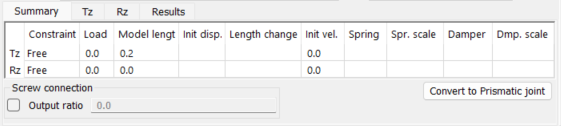
\includegraphics[trim=255 10 2 15,clip,width=0.34\textwidth]{\ReferenceImg/prp/cylindric-joint-1}}
  \end{picture}
\end{wrapfigure}

You can easily convert a Cylindric joint to a
\protect\hyperlink{prismatic-joint}{\sl Prismatic joint} by using the
\textbf{Convert to Prismatic joint} button in {\sl Summary} tab of the
Cylindric joint Property Editor panel (shown to the right).
The {\sl Tz} properties will then be transferred to the Prismatic joint,
whereas the {\sl Rz} properties of course will be lost.

Similaraly, a Prismatic joint will have a
\textbf{Convert to Cylindric joint} button in its {\sl Summary} tab,
which will add an (initially {\sl Free}) {\sl Rz} DOF.


\subsubsection{Cam joint}

\IconTextFirst{camJoint}{
  A cam joint has six unconstrained DOFs that allow the slave triad (a.k.a.
  the {\sl follower}) to move over a curved surface (the {\sl cam surface}).
  The cam surface is defined by a curve consisting of three-point circular arcs.
  Each arc is defined by the location of three master triads,
  also called the {\sl cam triads}.
  A cam joint must consist of one follower triad and at least three cam triads.
  See also the \FedemTGuide{Section 6.3.3, "Cam joint"}.}

It is recommended to use at least one arc segment per quarter of a circle
to make the solution more stable.
This means you will need at least eight master/cam triads for a complete circle.

\Tip{You can use the same cam triads in several different cam joints, making it
  possible to constrain several follower triads to the same cam surface.}

\noindent
\begin{minipage}{0.67\textwidth}
  \raggedright
  An example cam joint is shown to the right.
  %
  \vskip2mm
  \begin{bulletlist}
    \setlength\itemsep{1mm}
  \item Slave/follower triad
  \item Master/cam triads
    (represented by the sets of $X$, $Y$ and $Z$-axes extending from the curve)
  \item Cam curve (represented by the curve)
  \end{bulletlist}
\end{minipage}% <--- the % is needed here to kill off spurious spacing
\hfill\begin{minipage}{0.22\textwidth}
  \begin{picture}(75,75)
    \put(0,-20){\includegraphics[width=\textwidth]{Figures/cam joint symbol}}
    \put(22,65){\Bullet{1}}
    \put(-7,33){\Bullet{2}}
    \put(45,-12){\Bullet{3}}
  \end{picture}
\end{minipage}

\subsubsection{\sl\textbf{Creating cam joints}}

The cam curve is defined by circular arcs and straight lines. Each three-point
arc is defined by three triads. If the triads are located on a straight line,
a straight line will be defined (circular arc with zero curvature).

To create a cam joint, complete the following steps:

\begin{enumerate}
\item
  Click the cam joint icon.
\item
  Select a position for a new follower triad, or select an existing triad.
\item
  Confirm by pressing Done. If an existing triad was selected,
  this triad will become the follower triad, otherwise a new triad is created.
\item
  Select a position for the first master, or select an existing triad.
  You can also select an existing cam curve.
\item
  Confirm by pressing Done. If an existing triad was selected,
  this triad will become the first cam triad, otherwise a new triad is created.
  If an existing cam curve was selected, the new cam joint is complete,
  and the selected cam surface will be used by the new follower triad.
\item
  Repeat steps 4 and 5 until a sufficient number of masters has been
  added. As you add triads, they will be oriented automatically to have
  sensible orientations related to the cam curve. The $Z$-direction is set
  to point along the cam curve, while the $X$-direction, considered to be
  ``up'', is calculated from the direction going from the master triad
  closest to the follower and to the follower triad.
\item
  To close the cam loop, add the first master triad as the last one.
\item
  Fedem tries to set sensible directions on the master triads created,
  but should any of the directions be inconvenient,
  rotate them using one of the tools to move mechanism elements.
  See \refSection{moving-mechanism-elements}{Moving mechanism elements}.
\end{enumerate}
\vskip\parskip
\begin{minipage}{0.6\textwidth}
  \raggedright
  \begin{itemize}
  \item[9.]
    Define the spring characteristics you need for the contact behavior,
    and assign them to the correct joint variables. Normally, a non-linear
    spring with a stiffness-deflection curve as shown in the picture to
    the right will provide a decent contact behavior when assigned to the
    $X$-translation DOF.
  \end{itemize}
\end{minipage}% <--- the % is needed here to kill off spurious spacing
\hfill\begin{minipage}{0.37\textwidth}
  \includegraphics[width=\textwidth]{Figures/4-3-4-CamJointStiffness}
\end{minipage}

\subsubsection{\sl\textbf{Local coordinate system}}

The local coordinate system for a cam joint has its origin on the cam
curve at a point calculated as the closest point to the follower; this
point is referred to as the {\sl contact point}. The local $X$-axis is
then defined to be perpendicular to the cam surface and the $Z$-axis
tangential to the cam curve. The orientation of the local coordinate
axes depends thus on the location of the contact point along the cam curve.

\subsubsection{\sl\textbf{Cam joint variables}}

Cam joints display all the six DOFs as joint variables in the Property
Editor panel, but have some restrictions on the {\sl Constraint Type}
setting that is unique for cam joints.
The only legal settings are {\sl Free} and {\sl Spring-Damper}.
The {\sl Fixed} and {\sl Prescribed} settings are not available because
the cam joint uses a different formulation than the other joints.

The three main joint variables, defined in the $X$-, $Y$- and $Z$-directions
of the cam joint's local coordinate system, are:

\begin{itemize}
\item{\sl X-position} :
  The distance from the contact point to the follower in the
  direction normal to the cam surface (the ``thickness'' direction).

\EnumTip{If no stiffness is assigned to the $X$-translation DOF,
  the whole cam joint will be completely ignored by the Dynamics Solver.
  This might be used as a simple tool to toggle a cam joint
  on and off during testing and modeling of complex models.
  The solver issues a warning when the $X$-translation spring is missing.}

\item{\sl Y-position} : The distance from the contact point to the follower
  in the direction tangential to the cam surface and normal to the cam curve
  (``width'' direction).

\item{\sl Z-position} : The distance along the cam curve from the first
  cam triad to the contact point (the slider variable).
\end{itemize}

You are also allowed to Spring-Damper constrain the rotational DOFs of
the cam joint. Such rotational stiffness/damping might be beneficial as
a stabilization tool in some cases.

\Warning{The rotational DOFs in a Cam joint are not suited for representing
  large rotations. However, this affects the solution only when
  some of these DOFs are Spring-Damper constrained.
  Therefore, when Spring-Damper constraining the rotational DOFs,
  you must ensure that the added stiffness is high enough to keep the rotations
  small, typically $R_x < 0.3$, $R_y < 0.6$ and $R_z < 3.0$ radians.
  If not, the solution will probably diverge.}

The initial values of the cam joint variables are interpreted differently
compared with the other joint types.
The {\sl Length/Angle in model} quantity is always zero for all variables,
regardless of the modeling position of the follower.
For the $T_x$ and $T_y$ DOFs, this means that the deflection is always
calculated as the distance from the contact point to the follower in the local
$X$- and $Y$-directions, respectively.
However, for the $T_z$, $R_x$, $R_y$ and $R_z$ DOFs, the deflection is measured
relative to the modeling position of the follower.
The stress free length/angle of any springs associated with these DOFs are then
also defined relative to these initial positions.

\Warning{If the follower is not within the contact domain of the cam joint
  (see \protect\hyperlink{cam-thickness-and-width}
  {\sl"Cam thickness and width as contact domain"} below)
  at the beginning of the first time step, the rotational springs as well as
  the slider spring, if any, are ignored throughout the simulation.
  This happens because the stress free length of these springs then are
  undefined. A warning is issued from the dynamics solver if this occurs.}

\subsubsection{\sl\textbf{Cam friction}}

The friction parameters for cam joints are the same as those for
prismatic joints with the exception of the equivalent force,
which is the sum of the $X$-spring and $X$-damper force in the cam joint.
The friction state depends on the slider variable only.

\SubSubSection{\sl\textbf{Cam thickness and width as contact domain}}
              {cam-thickness-and-width}

\begin{wrapfigure}[3]{r}{0.4\textwidth}
  \vspace{-4.5mm}
  \includegraphics[width=0.4\textwidth]{Figures/4-JointPropCamFields}
\end{wrapfigure}

The thickness and width parameters shown in the Property Editor panel
define a rectangular domain in the $XY$-plane of the local coordinate system,
and is used to determine whether it is necessary to test if the follower
is in contact or not.
The springs and dampers associated with joint variables are activated only when
the follower is located within the distance {\sl Thickness}/2 from the cam curve
in the local $X$-direction and within the distance {\sl Width}/2 in the local
$Y$-direction. Use of a reasonable thickness is of great importance
to ensure that the contact springs are attached to the correct cam segment
(a cam segment is the part of a cam curve between two triads).
One should avoid having the cam thickness so large that two cam segment have
overlapping contact domains.

\Caution{When assigning highly non-linear spring characteristics
  to the cam joint variables to model contact behavior, it is often necessary to
  assign some associated damping to reduce fictitious oscillations due to sudden
  activation and deactivation of contact spring forces.
  A constant damping coefficient is then sufficient as long as the follower
  is within the contact domain throughout the simulation.
  However, if the follower enters the contact domain once or several times
  during the simulation, numerical instabilities may occur due to the sudden
  activation of the joint variable dampers, because they are active
  only when the follower is within the contact domain.
  To avoid this, it might be necessary to scale the damping coefficient
  with a function (see \refSection{damper-properties}{Damper properties}),
  that varies gradually from zero as the follower enters the contact domain,
  to one as the contact stiffness is activated.}

\subsubsection{\sl\textbf{Radial contact springs}}

By enabling the {\sl Use radial stiffness} toggle, the springs
associated with the $X$- and $Y$-variables are referred to local polar
coordinates in the $XY$-plane instead. Thus, the $X$-coordinate is then the
radial distance from the cam curve to the follower, and the $Y$-coordinate
is the angle between the local Cartesian $X$-axis and the axis extending
from the contact point through the follower. The contact domain will
consequently be a circular cylinder instead of a rectangular one, and
the {\sl Thickness} and {\sl Width} parameters above will now define
the radial and the angular (in degrees) extension of the contact domain.
This can be used to simulate contact in pipes, etc.

\Note{The {\rm Use radial stiffness} toggle does not affect the dampers (if any)
  that are assigned to the joint variables. They are still applied in the local
  Cartesian coordinate system. It is therefore advisable to apply the same
  damping characteristics to the $X$- and $Y$-variables when using radial
  stiffness, to ensure a proper damping behavior in the cam joint.}

\subsubsection{\sl\textbf{Cam with spherical or cylindrical follower}}

Often the follower in a cam joint should have a spherical or cylindrical
shape. Below, we describe how such behaviour can be modelled.

The radius of the sphere or cylinder must be entered as an
{\sl Initial stress free length} for the spring in the $X$-translation DOF
(see \refSection{spring-properties}{Spring properties}).
A normal contact stiffness function can then be used.
The {\sl Thickness} of the cam must also be set to a value greater than
the roller radius in this case.

This will work as expected as long as the follower never is in contact
with the cam curve at more than one location simultaneously.
This means that the follower can not pass the inside of a v-shaped cam curve,
or curve segments that have a radius equal to, or less than the roller radius.
By trying to do so, the numerical simulation will normally fail to converge
when two simultaneous contact locations would be expected.

If the cam curve to be modeled has this kind of features, you will need to model
the different parts of the contact curve as {\sl separate cam joints} instead,
and re-use the same triad as follower in all those cam joints.
You will also have to set them up with the same contact spring
characteristics and {\sl Initial Stress free length}.

\Caution{When using a radius on the follower, even small discontinuities of the
  cam tangent between curve segments might result in a v-shaped curve.
  The v's can cause numerical problems if the follower is on the inside of it.}
